\documentclass{standalone}

\usepackage{tikz}
\usetikzlibrary{shapes.multipart, calc, arrows}

\begin{document}
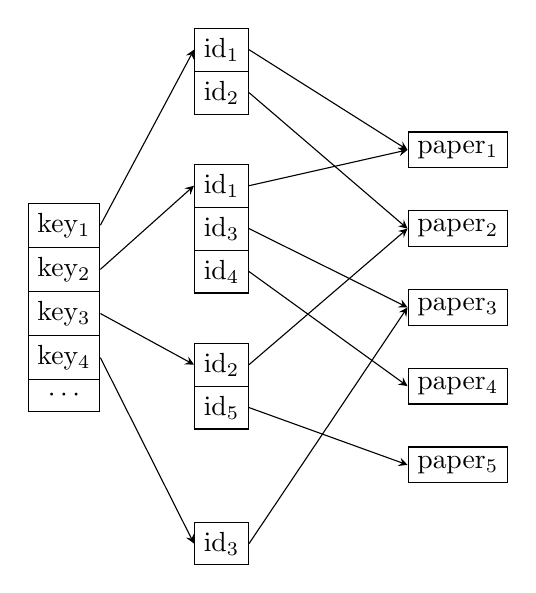
\begin{tikzpicture}
    \node[
        rectangle split,
        rectangle split parts = 5,
        text centered,
        draw,
        fill = none
    ] (key) at (0, 0) {
        key\textsubscript{1}
        \nodepart{two} key\textsubscript{2}
        \nodepart{three} key\textsubscript{3}
        \nodepart{four} key\textsubscript{4}
        \nodepart{five} $\cdots$
    };

    \node[
        rectangle split,
        rectangle split parts = 2,
        text centered,
        draw,
        fill = none
    ] (id1) at (2, 3) {id\textsubscript{1} \nodepart{two} id\textsubscript{2}};

    \node[
        rectangle split,
        rectangle split parts = 3,
        text centered,
        draw,
        fill = none
    ] (id2) at (2, 1) {id\textsubscript{1} \nodepart{two} id\textsubscript{3} \nodepart{three} id\textsubscript{4}};

    \node[
        rectangle split,
        rectangle split parts = 2,
        text centered,
        draw,
        fill = none
    ] (id3) at (2, -1) {id\textsubscript{2} \nodepart{two} id\textsubscript{5}};

    \node[
        rectangle,
        draw,
        fill = none
    ] (id4) at (2, -3) {id\textsubscript{3}};

    \node[
        rectangle,
        draw,
        fill = none
    ] (paper1) at (5, 2) {paper\textsubscript{1}};

    \node[
        rectangle,
        draw,
        fill = none
    ] (paper2) at (5, 1) {paper\textsubscript{2}};

    \node[
        rectangle,
        draw,
        fill = none
    ] (paper3) at (5, 0) {paper\textsubscript{3}};

    \node[
        rectangle,
        draw,
        fill = none
    ] (paper4) at (5, -1) {paper\textsubscript{4}};

    \node[
        rectangle,
        draw,
        fill = none
    ] (paper5) at (5, -2) {paper\textsubscript{5}};

    \path[->, -stealth]
    (key.one east) edge (id1.one west)
    (key.two east) edge (id2.one west)
    (key.three east) edge (id3.one west)
    (key.four east) edge (id4.west)

    (id1.one east) edge (paper1.west)
    (id1.two east) edge (paper2.west)

    (id2.one east) edge (paper1.west)
    (id2.two east) edge (paper3.west)
    (id2.three east) edge (paper4.west)

    (id3.one east) edge (paper2.west)
    (id3.two east) edge (paper5.west)

    (id4.east) edge (paper3.west)
    ;
\end{tikzpicture}
\end{document}

